% \newcommand{\subsubsubsection}[1]{\paragraph{#1}\mbox{}\newline}
% \setcounter{secnumdepth}{4}
% \setcounter{tocdepth}{4}


%TODO: Please DO NOT RESOLVE the comments unless you are 100% sure everything related to the comment is resolved, as they can't be retrieved.
%TODO: VERY VERY IMPORTANT: talk to people in our group to make a decision on understanding of the "lack of variety"  that is shown in the comment on line 276 of this latex file. This will cause quite a few changes in the report but it is a very important concept to clarify to avoid burning ourselves. Read all the comments Mike made in the relevant sections first.
%TODO: VERY IMPORTANT: another potential self burn area. Clarify with Rudolfs about Ostrom's Principles after looking at all the comments Mike has made in that section.
%TODO: add in rule distance calculation explanation? It's kinda primitive though
%TODO: President by Andrzej, do talk about disaster prediction
%DONE I THINK: Toby to finish all foraging related stuff (IIFO and End of turn)
%TODO: add in the use of disaster prediction somewhere if we can?
%TODO: to finish IITO and gifting, sneak in disaster prediction if possible - This is done except for the disaster prediction part. Not sure how to add it though, but feel free if you have an idea how.
%TODO: clear up all the TODO's scattered around in this latex file.


\chapter{Team 4 Agent Design}   \label{chap:team4}
Given that our team invested a lot of time in ensuring feature richness and stability of the infrastructure, we were left with a short time-frame for our agent's implementation and design. Therefore, at times we had to make decisions that guaranteed canny usability, rather than sophistication. For some actions, our agent relies on other teams' agents with different strengths to perform well. 

\section{Agent overview}
An agent uses the interface that is defined in the infrastructure. In order to define custom behaviours for our agent, we override or extend the base agent (\texttt{baseclient.go}) functions which implement the defined interface. The main idea we have for our agent is that it has internal fields that aid the decision-making process for the actions it performs. Of all the internal fields, we define internal parameters as information that describes the agent itself, namely \texttt{Greediness}, \texttt{Selfishness}, \texttt{Fairness}, \texttt{Collaboration} and \texttt{RiskTaking}, all of which have decimal values between 0 and 1. The agent stores observations, histories as well as other necessary information such as its trust in others. These internal fields will be discussed in more detail in the following dedicated sections. %TODO: add in evolutionary economic theory background for agent personality


% TODO: Chapter reference
An agent can be elected in one or more positions of power inside the IIGO session. Each role has the ability to perform certain actions, specified in chapter 7 (?). From an infrastructure standpoint, these actions are implemented as overridable functions in the same fashion as previously discussed for the base agent. Although the code was design to differentiate a commoner agent and roles in separate structs, they all share read and write access to the internal fields of each other through pointers. In other words, an agent is always a commoner agent, and a commoner agent can be elected one or more role(s) at the same time.

\section{Opinion formation -- Trust}
\label{sec:team4:trust}
Trust is the score $[0..1]$, which represents the agent's opinion towards fellow agents in the game. This metric helps it in making decisions throughout the game based on how trustworthy, helpful or friendly it believes other agents were. This generic opinion about an island is formed dynamically based on three recurring observations:
\begin{itemize}
    \item The gifts received from the island during the IITO sessions.
    \item The outcome of monitoring positions-of-power when conducted as a part of the accountability cycle.
    \item The evaluation of IIGO actions history, only available to the Judge. This is further explained in Section \ref{subsec:team4:judge}
\end{itemize}
Those observations allow the agent to quantitatively reason about both friendliness of other islands towards it, as well as how closely they follow the rules in play.

The average trust score is forced at a value of $0.5$. Such normalisation ensures that the trust is always balanced throughout the game. It prevents the inflation of trust in a scenario where several islands decide to exchange gifts with the agent. Furthermore, the number of resources gifted will be a deciding factor when updating the trust metrics.

Some decisions made by our agent can be altered based on the trust score towards certain islands. During elections, if the trust of an island is lower than a specified threshold, the agent will never cast its vote in favour of it. Similarly, if holding the role of Judge, it will choose not to act upon its power to pardon the island with a low trust score.

On the other hand, if the agent holds a good opinion about an island, it may choose to favour it by providing or even deciding to  pardon it from a sanction.


\section{IIGO}
\subsection{Commoner Agent} \label{commoneragent}
At the start of any IIGO, each (commoner) agent is promped by the president to report how many resources it has. Our agent overrides its reporting behaviour to account for several internal factors, as further discussed in subsection \ref{reportresources}. The president uses this information to set a taxation amount according to each agent's self-report, notifying them of the tax demanded. Each (commoner) agent can later send a request for the specific amount of resources it aims to retrieve from the Common Pool (an allocation request) to the President. Upon receiving a response by the President on the actual amount that was granted, the agent is allowed to access the Common Pool. The actions concerning requesting and taking allocations are overridden, as part of the agent strategy. Due to a design decision, the action for taking allocations and paying tax do not happen within the IIGO session, it happens after all organisations are run, inside the \texttt{EndOfTurn} session.

\subsubsection{Report Resources} \label{reportresources}
When reporting its resources, our agent uses a weighted linear combination of some of its internal fields. The weighting of each parameter is defined as an array of real values called "importance" and stored in an \texttt{importance} vector. The linear combination outputs a scaling factor to divide to the actual resources our agent has, as shown in \eqref{linear_comb}, in order to compute a untruthful amount to report to the President. The parameters used are \texttt{greediness}, \texttt{selfishness}, \texttt{fairness}, \texttt{collaboration}, \texttt{riskTaking} and trust in the current president (all values are between 0 and 1). Some fields are associated with negative weights as they should logically negatively impact the scaling factor. The greater the absolute value of a weight, the bigger impact it has on the scaling factor.

\begin{equation}\label{linear_comb}
    \begin{bmatrix}
        w_{1}& w_{2}& w_{3}& w_{4}& w_{5}& w_{6}
    \end{bmatrix}
    \cdot
    \begin{bmatrix}
    Greediness \\ 
    Selfishness \\ 
    Fairness \\ 
    Collaboration \\ 
    RiskTaking \\
    TrustScore_{President}
    \end{bmatrix}
    = Scaling\:Factor
\end{equation}

To decide when to lie, the scaling factor is firstly compared to a preset threshold. If the scaling factor is greater, then the needed resources amount is divided by 
\begin{equation}
    [1 + (Scaling\:Factor - Preset\:Threshold)]
\end{equation} 
This conditional statement makes sure that the scaling factor is not always applied, ensuring that our agent will lie on its resources only when deemed a good strategy.

\subsubsection{Paying Tax Contribution}
%write about this and the lying mechanics
The \texttt{GetTaxContribution()} function returns the amount an agent is paying in tax. Similarly to resource reporting, the tax amount is modified by a scaling factor applied only when greater than a preset threshold, as shown in the following equation: 
\begin{equation}
    [1 + (Scaling \: Factor - Preset \: Threshold)]
\end{equation}
Based on the preset weighting for internal parameters, this situation is likely to arise when the \texttt{Collaboration} of our agent is high. In addition, the scaling factor is not applied when the tax demanded is more than $\frac{1}{5}$ of the agent's resources. This prevents it from generously giving out most that it has.

\subsubsection{Requesting Allocation}\label{subsubsection:CommonPoolResourceRequest()}
The aforementioned action of requesting resources from the common pool is implemented in the \texttt{CommonPoolResourceRequest()} function. When requesting an allocation, our agent first decides what it needs. When not in a critical state, the needed resources are usually a multiple of the basic needs, namely the cost of living plus the critical threshold. This amount is decided so that the agent always takes more from the Common Pool than their definite expenses in the next turn. If critical, the agent will ask for a bigger multiple of the basic needs. This design choice maps the following logic conclusion that the agent draws from the history of the game: if the a smaller multiple when made the agent critical, it must take more to invert the negative trend in resources. In order to avoid draining the Common Pool, our design enforces that what our island needs must not exceed the amount of resources in the Common Pool divided by the number of agents alive. This is to avoid our agent selfishly monopolising the Common Pool resources.

\subsection{President}
\label{subsec:team4:president}
Our agent implements a budget-conscious and rule-obeying President. The main changes, compared to the basic implementation include taxation and resource allocation considerations.

\subsubsection{Tax distribution}
When deciding tax amounts for the different island, the President considers the following variables:
\begin{itemize}
    \item amount of resources in the common pool
    \item the financial status of the island
    \item predicted disaster time and magnitude.
\end{itemize}

The President will abstain from setting taxation for islands in a critical state or in a situation when the resources in the common pool can fully mitigate the predicted damage caused by the next disaster. 

Similarly, when the common pool cannot mitigate the next disaster, the President will set taxation for all non-critical island to bring the common pool back to the safe level. In this case, the taxation amount will be higher the sooner the disaster is predicted to occur.

\subsubsection{Common pool resource redistribution}
In order to fairly redistribute the resources placed in the common pool, the President primarily considers the financial status of an island. In other words, the priority in access to the common pool is given to islands in the critical state. 

To ensure the largest possible satisfaction within the archipelago, the islands with smaller requests are given priority. This decision ensures that the highest possible number of agents will be satisfied with their allocation.

The President is also reluctant to allow any resource allocations if the disaster is predicted to occur soon. This, combined with the tax policy, ensures lower damages to the archipelago in the case of disaster.


\subsection{Judge}
\label{subsec:team4:judge}
The Judge implementation provided by our agent can be described as \emph{honest, but curious}. In other words, it follows the rules currently in play, and follows its obligations, however, it extracts the information exclusive to Judge to reason about other agents in the game. An example of such actions is explained in greater detail below in this Section.

The judiciary functions overloaded from the \texttt{basejudge} implementation are:
\begin{itemize}
    \item \texttt{InspectHistory}, which examines rule violations of all the agents.
    \item \texttt{GetPardonedIslands}, which considers reducing the sanctions for some agents at judges discretion.
    \item \texttt{CallPresidentElection}, which initialises \emph{transfer-of-power} of the executive branch.
\end{itemize}
An explanation of the implementation of those functions is presented below.

\subsubsection{IIGO history inspection}
\label{subsubsec:team4:judge:inspect_history}
In the basic implementation, a history of IIGO actions of all the agents is passed to the Judge for inspection, which could become grounds for introducing economic sanctions for non-rule-obeying players. 

Judge truthfully evaluates and reports the rule violations of each of the agents, just as the \texttt{basejudge}. However, it also extracts and saves the information about the private resource pools of all the agents, taxes they were expected to pay, as well as the actual amount paid to the common pool. Additionally, it stores the \texttt{LawfulnessRatio} of each agent, which can be written as:


\begin{equation}
    lawfulness_{i} = \frac{number\:of\:rules\:obeyed\:by\:the\:agent_{i}}{total\:number\:of\:rules\:inspected\:by\:the\:judge\:for\:agent_{i}}
\end{equation}

where $agent_{i}$ is denotes $i^{th}$ agent in the game.  

The \texttt{LawfulnessRatio} is then used to update our agents' trust towards other islands, thus influencing decisions in different parts of the game. 

\subsubsection{Consideration of pardons}
Compared to the \texttt{basejudge}, which does not grant any pardons and requires islands to pay economic sanctions in full, our implementation of the Judge allows for the pardoning of certain islands. We consider three parameters when deciding whether and the island could be pardoned:

\begin{enumerate}
    \item The severity of the sanction - only sanctions lower than specified severity level can be considered to be pardoned. This ensures that our Judge never pardons an island, who notoriously breaks the rules of the game and gets sanctioned for it.
    \item Time served on the sanction - the Judge will only remove the sanction if at least the specified number of turns has been served by the island. This still allows us to have a punishment for not obeying the rules but also ensures that an island can begin to contribute again earlier.
    \item Trust towards the island sanctioned - only islands, which are considered trustworthy by our agent can be pardoned. The threshold is tuned by an internal parameter of our agent.
\end{enumerate}

An island can be pardoned by our implementation of Judge only if they meet all three requirements presented above. 


\subsubsection{Presidential elections}
The \texttt{basejudge} implementation called an election every three turns, no matter how long the presidential term was. Our Judge implementation improves on that by calling an election only under two conditions:
\begin{enumerate}
    \item The term of the president has ended.
    \item The president did not fulfil its obligations and was dishonest while holding the executive office. It is decided based on the monitoring results coming from the accountability cycle.
\end{enumerate}

This implementation could be further improved to facilitate the \emph{trust} metrics, explained in Section~\ref{sec:team4:trust}. An example of such an improvement would be allowing the president to hold the office longer than its turn if he is most trustworthy according to our internal \emph{trust} metrics.

\subsection{Speaker}
Given the Speaker's role of deciding agendas and announcing the results of voting, the only viable customisation option in making our custom Speaker seemed to be via implementing corruption - in other words, rigging voting results. Other than the obvious reason of avoiding the risk of getting sanctions, we decided against implementing this function into the Speaker's role because in an actual governmental environment, while misprints have occurred and on occasion shaped past history, announcing false results are a very noticeable and easily rectifiable offense. This would be in the disinterest of either honest or dishonest agents. On this note and the following point, it could be said that our Speaker implementation can be described as \emph{honorable and efficient}.

\subsubsection{Action prioritisation}

Our Speaker implementation builds upon the \texttt{baseSpeaker} on a key point: partitioning of budget. The Speaker prioritises the proper running of IIGO in the case of a low budget situation by prioritising its actions according to the rules in play, reflecting the priorities decided by the archipelago. This is done not by changing the actual running order of IIGO (which would require altering the orchestration) but rather enabling/disabling certain actions based on their priorities and cost. Prioritising actions where rules are in play would stop the speaker from performing non-moderated actions instead of actions relating to rules that are still in play. This function is crucial due to the following reasons:
\begin{itemize}
    \item Not performing monitored actions will result in sanctions, harming the agent's resource pool.
    \item The rules are a representation of the archipelago's expectations, thus not following said priorities is a sign of incompetence - damaging the agent's reputation.
\end{itemize}
Since these reasons are applicable regardless of honesty, these mechanics are always implemented regardless of agent type.

\section{IIFO}\label{sec:team4:IIFO}
%I recommend that we write in the order of function execution order. (the end of turn functions that are related to IIFO should be written inside the EndOfTurn section)Only mention the functions that are worth mentioning. For execution order check the ./doc/EXECUTION_ORDER.md file in the SOMAS repo -- Mike

\subsection{Making Disaster Prediction}
The agent makes predictions about future disasters by getting the mean coordinates, magnitude and number of turns per disaster (i.e. $\frac{1}{freq}$) from the previous disasters. It then computes a \texttt{confidence} score based on these mean values. The \texttt{confidence} score has a range between 0\% and 100\%. The sum of square of difference between the actual value and the mean value for each of the 4 prediction values types(coordinate x, coordinate y, magnitude and turns) is calculated as below:
\begin{equation}
    total = \sum_{i=1}^{len(past\_disasters)}(Value_i - Mean_i)^2
\end{equation}

The above is done for each of the 4 prediction values types. This returns a measurement of the distance between the predicted value (mean value) and the corresponding past disasters' values. The computed sum of square of difference (a measure of distance) is normalised with a max distance (see equations \ref{max_distance:1} to \ref{max_distance:3}) for each of the 4 value types, 100\% minus this percentage value is the \texttt{confidence} score. The \texttt{confidence} score for the prediction is the average of the 4 \texttt{confidence} scores.

Note that the Central Limit Theorem can be applied in this calculations since we assume different disasters are independent. Namely, the higher the distance between a prediction and samples, the less likely it is for this prediction to be true. And with the CLT assumption, the underlying random variables of the value types (uniform RV for coordinates, geometric RV for both magnitude and turns) do not matter. The calculation of the unique preset threshold is below:
\begin{equation}\label{max_distance:1}
    distance_1 = \sum_{i=1}^{len(past\_disasters)}(ValueMax - Mean_i)^2
\end{equation}
\begin{equation}\label{max_distance:2}
    distance_2 = \sum_{i=1}^{len(past\_disasters)}(ValueMin - Mean_i)^2
\end{equation}
\begin{equation}\label{max_distance:3}
    max\: distance = max (distance_1, distance_2)
\end{equation}

By doing the above unique threshold calculation for each value type, we are setting the predicted values out of bounds to have confidence 0\%. (Note: ValueMax and ValueMin are set in game config)

\subsubsection{Making prediction based on other agents' predictions}
Our agent then receives prediction information from all other agent that sent their information to us. A weighted average (based on trust) of these prediction values are calculated to form our final prediction values.

%Theoretically, We would use  a normal distribution to approximate the sampling distribution of the disaster random variable, which is assumed to be independent across turns, justified by the Central Limit Theorem. And by feeding  calculation approximated to be 


% Foraging functions %
\subsection{Sharing foraging information} \label{sec:team4:IIFO:forage}
IIFO also contains the ability to communicate about the foraging information. As we will go further into in Section~\ref{sec:team4:forage},
we choose to overload both MakeForageInfo and ReceiveForageInfo. In the receive function, we store the received values to a map to be used later when making a decision on which foraging method to go for. 

As we use the foraging information from other teams, our island will also communicate our results to the others. However, we only share with islands that shared with us in the previous round, as well as the island that we trust. Our island is completely truthful for this part and will always report which foraging method we went for, as well as how many resources it generated.

\subsection{IITO}
%(put and modify this to fit it somewhere in this section) If our agent is not in a critical state, it requests extra resources in addition to its own wanted resources in an intention to gift to other agents to earn their trust. If this allocation request is approved by the President, it proceeds with the gifting. These gifted resources are given on top of the normal gifts if there are any.
% some rough comments about IITO from Fabio: gifting pool is the key concept. same as president for allocation. Prioritise agents that are critical. Look at our selfishness and current resources. Help critical first(full amount no matter the trust). If not critical, only gift if trust > 0.5
In IITO we handle the process of sending, receiving, and requesting gifts.
Our island has an internal wealth goal which is calculated using our internal greediness and selflessness parameters. If our private pool is smaller than our wealth goal we ask for gifts from the other islands. The amount we ask for is related to the difference between the private pool and wealth goal. If we are in a critical state, however, we ask every island for two times the resources we estimate to be a safe resource level in the hope that at least one island will support us. 

When an island requests a gift from us we first check how many resources we can spare. This is once again calculated by taking the difference between the private pool and the wealth goal. We also look into its trustworthiness. If the island is critical, we prioritise that island. After that, we only return the gift relative to their trustworthiness. 
In addition, when we request allocation in IIGO, we request a bit extra which we gift to other islands in the hope that it will increase our reputation. This is only done if the president permits us to take the extra resources. 


 

\section{End of Turn}
\subsection{Taking Allocation}
This RequestAllocation() function for taking allocation from the Common Pool. After running all of the organisation sessions, the agent then calculates what it wants based on what it needs, and takes what it wants from the Common Pool. A scaling factor is calculated using a linear combination of weights and internal fields. When the scaling factor is above a preset threshold, it is applied similar to in Section~\ref{subsubsection:CommonPoolResourceRequest()}.  %talking about scaling factor calculation briefly, the detailed explanation is already done in ResourceReport. %%We use a linear combination of some of the agent's internal fields, and weights (put inside an \texttt{importance} vector) we set for each of the chosen internal fields to obtain a scaling factor to multiply the needed resources with. The parameters used are \texttt{greediness}, \texttt{selfishness}, \texttt{fairness}, \texttt{collaboration}, \texttt{riskTaking} and trust in the current president (all values are between 0 and 1). The weights have real values. For this particular function, we set the weights to be $5, 5, -5, -5, 1, 5$ respectively. The fields with negative weights negatively impact the scaling factor and vice versa. We deem riskTaking less important than other fields in the calculation of this function's scaling factor. The scaling factor is then compared to a preset threshold. If the scaling factor is greater, then the needed resources amount is multiplied by 1 plus the difference between the scaling factor and the preset threshold. The threshold is there to make sure that the scaling factor is not applied all the time, as we don't want our agent to take more than what it needs all the time.

\subsection{Forage} \label{sec:team4:forage}
As mentioned at the start of the chapter, due to the interest of time, our foraging strategy relies on other islands to make intelligent decisions about the foraging strategy. In short, rather than looking at the game configurations to try to intelligently figure out which method to go for and how many resources to generate, we look at other teams' return ratios to decide for ourselves. As will be discovered in the simulation section (\ref{sec:team4:simulation}), our foraging strategy works very well against the other islands created by the other teams, but not so well when we simulate six of our own islands.  

Our foraging strategy is split into two sections. Managing foraging communications is stored inside IIFO.go and our foraging decisions are stored inside Foraging.go

As mentioned in Section~\ref{sec:team4:IIFO:forage}, 
the foraging is split into two parts, decision, and return. In the return, we store the results we receive into an array so that we can later use them in the decision making. This is also what we do inside IIFO when we receive the foraging results from the other teams. 

To decide whether to go fishing or to hunt deer the island looks at both its return history as well as looking at the return results received from the other teams. Our island does this is by calculating the return ratio of each island over the past three turns as well as our own. These ratios are then compounded into two separate values, the compounded ratio for deer hunting and the compounded ratio for fishing.  We then pick the foraging method that has the greatest compound ratio. 

How the island chooses to share its foraging results with other islands was described earlier in Section~\ref{sec:team4:IIFO:forage}. 


\section{Simulation}    \label{sec:team4:simulation}



\subsection{Introduction}
Three different initial personality configurations were defined -
\emph{honest} , \emph{moderate} and \emph{dishonest} - in order to simulate how internal parameters would impact the agent's performance and interaction with the other teams.
These agents are designed to adapt their decision-making processes throughout the game, and each of these different personalities drew interesting hypotheses and observations about how a single agent would affect other agents and the system as a whole. This will be further discussed in Section~\ref{ResultSummary}. 

The team decided to test both the interactions in the archipelago when populated by our agent and the default clients developed by other teams (discussed in Section~\ref{againstothers} \nameref{againstothers}) as well as the interactions when only populated by instances of our agent (discussed in Section~\ref{againstself} \nameref{againstself}). These simulation efforts have been made to investigate the effectiveness of the agent's strategy, the system's response to the lack of strategy variance, as well as the ability of the agents to react to this issue.

\subsection{Multi-agent simulations} \label{againstothers}
\subsubsection{Honest Client} \label{honestAO}
The \emph{honest} client has been carefully designed as an agent who would start the game complying to rules, offering help when possible and contributing to the common pool with more taxes when the agent is in abundant wealth. However, the personality of the agent adapts to the environment as it self-organises its strategy based on fellow agents. An irrefutable sign of great flexibility of this agent configuration is the presence of sanctions in its IIGO Report as shown in Figure~\ref{fig:IIGOHO}.
The figure testifies that the agent occasionally breaking the rules - adopting a change in strategy in order to adapt to the strategies of other agents. It still maintains a fair and collaborative approach throughout the whole game, getting involved in transactions during the IITO (Figure~\ref{fig:TransactionsHO}) and contributing to the common pool. As shown in the Resources Plot in Figure~\ref{fig:ResourcesHO} , where the agent is represented by the cyan curve, more than once there is a peak in resources that steeply decreases on the following turn, as the agent generously providing gifts to the agents in need and sometimes also paying slightly more taxes in the common pool. From a design standpoint the team opted for an implementation that would prioritise gifts over over-contributions to the common pool. This decision comes from the consideration that a dishonest agent would counter our efforts in distributing resources to fellow agents. Therefore, prioritising gifting avoids this problem by allowing our agent to deliberately allocate its resources surplus to other islands. The agent acts even more magnanimously with islands in a critical state. This behaviour is clearly noticeable in disaster recovery.
\begin{figure}[H]
\centering
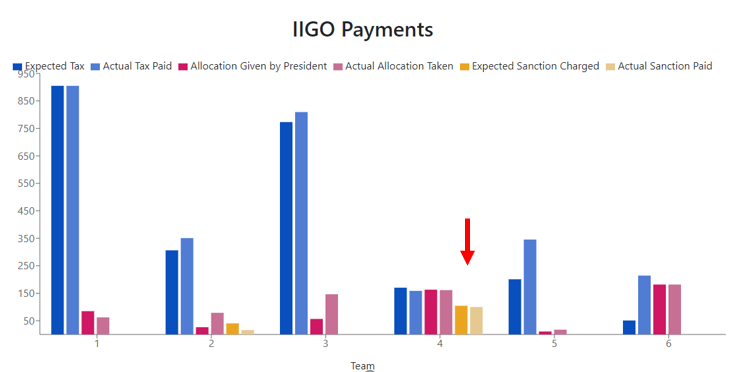
\includegraphics[scale=0.6]{12_team4_agentdesign/images/IIGOHO.PNG}
\caption{IIGO Payments For Honest Client Versus Other Teams.}
\label{fig:IIGOHO}
\end{figure}

\begin{figure}[H]
\centering
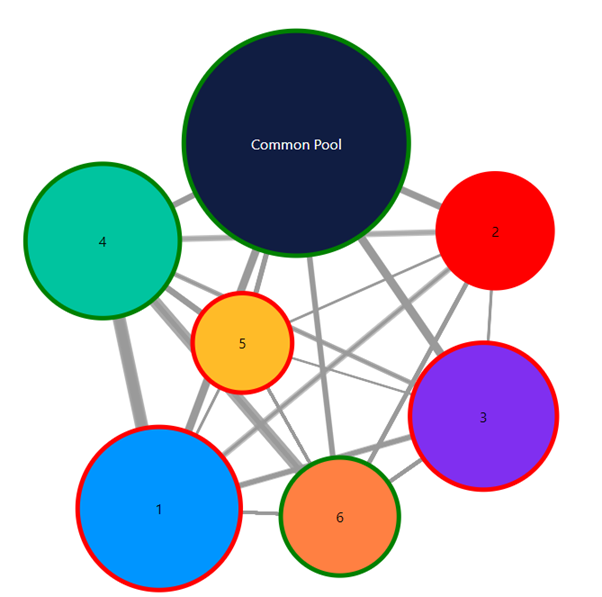
\includegraphics[scale=0.4]{12_team4_agentdesign/images/TransactionsHO.png}
\caption{Transactions For Honest Client Versus Other Teams.}
\label{fig:TransactionsHO}
\end{figure}
\begin{figure}[H]
\centering
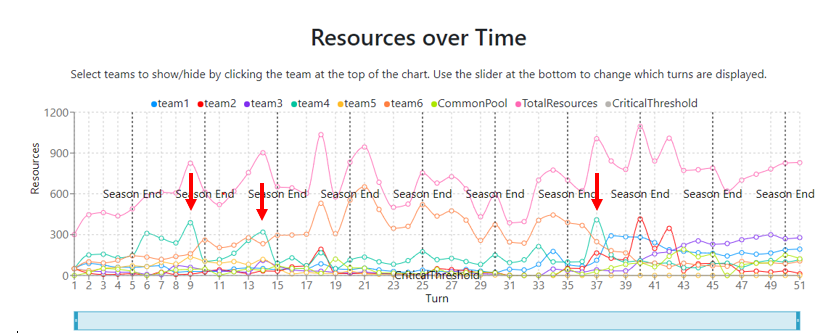
\includegraphics[scale=0.7]{12_team4_agentdesign/images/ResourcesHO.PNG}
\caption{Resources Plot For Honest Client Versus Other Teams.}
\label{fig:ResourcesHO}
\end{figure}

\subsubsection{Moderate Client} \label{moderateAO}
The \emph{moderate} client is configured specifically to start the game with an internal set of parameters that would allow it to score values as close as possible to thresholds in each decision making matrix calculation. The team opted for such a design choice in order to maximise the agent's response time to the environment, making it much more flexible than its two counterparts, who take a longer time to modify their strategy. As a Moderate client was simulated against other teams, the team noticed that it would perform very similarly as the Honest agent, as the other teams were always run on a "honest-like" configuration. Similarly, it would quickly turn its behaviour to dishonest when running against dishonest-like implementations of other teams' agents.

\subsubsection{Dishonest Client}
The \emph{dishonest} client, aptly named, is designed to take advantage of a large amount of common resources without collaborating with others and systematically abusing positions of power to gain economical advantages. The yielded results highlighted an interesting behaviour of the system and of other agents. As per design, the system is not flexible enough to mitigate such radical and rogue behaviour, resulting in a complete dominance of the dishonest agent. The agent proceeds to appropriate of all resources from the common pool and mercilessly watch other islands die, as profiled in Figure \ref{fig:ResourcesDO}. Eventually unable to survive without the collective help to mitigate disasters, it slowly meets its demise. The other agents do not reach a level of understanding of the game that allows them to comprehend what is going on and try to mitigate it by enforcing more severe rules. It must also be said that the system itself does not allow any hard enforcement, making it impossible for other agents to counter-attack a fully dishonest and selfish strategy, which disregards sanctions and taxes. Given these findings, dishonesty might seem like a dominant strategy as the agent survives the longest, securing all resources for itself. However, the long term dilemma imposes that islands must collaborate to survive for long periods. The dominance of this strategy is further refuted by the simulations performed in subsection \ref{dishonestAD}.

\begin{figure}[H]
\centering
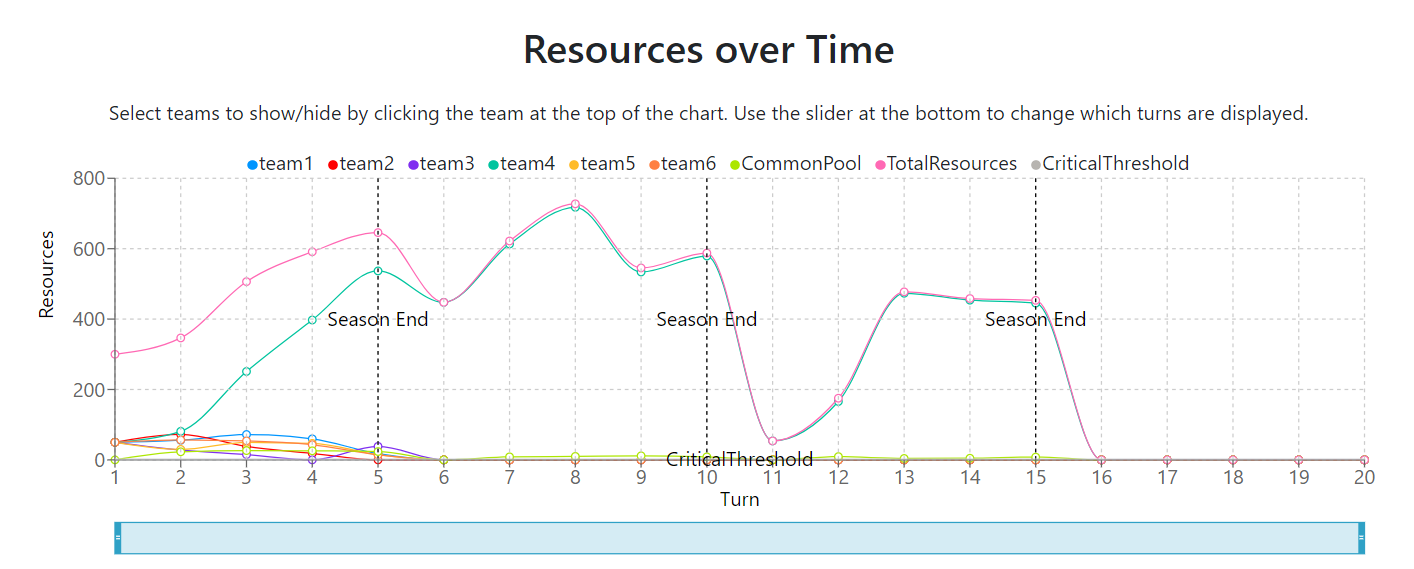
\includegraphics[scale=0.4]{12_team4_agentdesign/images/ResourcesDO.png}
\caption{Resources Plot For Dishonest Client Versus Other Teams.}
\label{fig:ResourcesDO}
\end{figure}

\subsection{Uni-Agent Simulations} \label{againstself}
Simulating our agent against instances of itself raised some interesting talking points. The main issue identified can be referred to as a \emph{lack of variety}, which encompasses the problem of populating the archipelago with islands that share the same "mindset"; therefore, approach dilemma from a unified prospective. This hypothesis was raised as an attempt to explain the poor results of uni-client simulations which have been observed not only when running team 4 agents against themselves, but also when other teams' agents were put against themselves under the uni-agent settings.

In all uni-agent simulations, the common pool was initialised to 1,000 resources, so that the agents could have enough resources to initialise running IIGO sessions.

\subsubsection{Honest Agents Only}
Populating the game with only honest clients provided a starting environment where all clients in the game are inclined to obey to rules and contribute a lot to the common pool in collective efforts. From this standpoint it makes sense that clients would build strong relations of trust and retain a high opinion of each other, as they treat each other with a fair and collaborative personality. Therefore in the evolution of the game, no agent undertakes any radical change of personality as was the case when our honest client was placed against other teams in subsection \ref{honestAO}. The IIGO Payments histogram in Figure \ref{fig:IIGOHH} nicely shows how the islands do not break any rule throughout the entire run.

It also manifests a very predictable behaviour of each honest agent that is perfectly in line with their design, such as paying more taxes than requested and taking less allocations than granted. The team identified this predictable behaviour as an example of \emph{lack of variety} that shows how agents with the same specification are not adaptive enough to survive in such a complex system that begs for a variety of strategies to be properly discovered and efficiently exploited.

\begin{figure}[H]
\centering
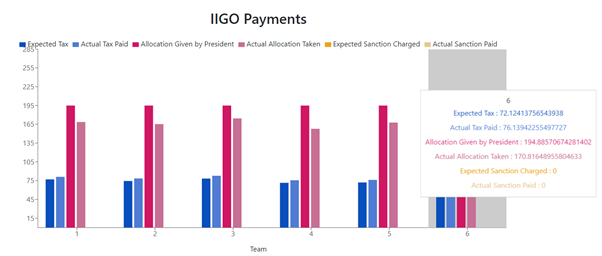
\includegraphics[scale=0.8]{12_team4_agentdesign/images/IIGOHH.png}
\caption{IIGO Payments For Honest Clients Only.}
\label{fig:IIGOHH}
\end{figure}

\subsubsection{Moderate Agents Only}
As presented in subsection \ref{moderateAO}, moderate agents are specifically designed to increase the variance in agent strategy. As a result, the \emph{lack of variety} issue should have been mitigated in a simulation where moderate agents face each other. After running the simulations, the clients have indeed acted far less predictably. Comparing Figure \ref{fig:IIGOMM} with the histogram plot shown in Figure \ref{fig:IIGOHH}, the breadth of a larger variety of game strategies can be observed. Namely, agent 2 and 3 show more dishonest traits, hence getting sanctions for performing illegal actions. Meanwhile, other clients take a more honest approach which replicates the ones observed by the honest clients. For other clients, like number 6, this honest strategy is less pronounced.

\begin{figure}[H]
\centering
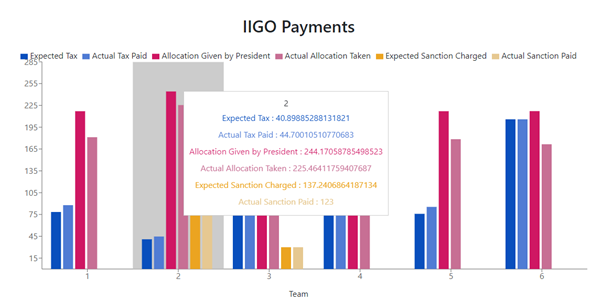
\includegraphics[scale=0.8]{12_team4_agentdesign/images/IIGOMM.png}
\caption{IIGO Payments For Moderate Clients Only.}
\label{fig:IIGOMM}
\end{figure}

Although the variance of agents strategy is significantly higher, clients still share the same underlying "mindset". This means that they define their whole personality using the same features, such as approaching tasks like foraging and power roles in the same way. Therefore, although the simulations ran show a slight improvement compared to "only honest" and "only dishonest" studies, they are far from producing a successful game like in multi-agent simulations. One of the main causes of this phenomenon was identified as the poor performance of actions that have been deliberately implemented in a simpler way in order to reduce the complexity of the agent. In particular, a foraging strategy in a well-performing multi-agent system may be to just replicate the foraging decision of the team that is economically strongest. However, in a uni-agent environment, this strategy  results in a group of agents mutually trusting their foraging strategy where nobody considers which one is actually the most profitable given the current circumstances.

Furthermore, features such as proposing rules is another good example of how lacking variety results in weaker archipelagos. This action enhances the ability of clients to adapt to the environment, crafting new rules as unexpected situations arise. If a client decides not to implement this feature in a multi-agent system, its effect on the adaptive capability of the archipelago will be almost fully mitigated by more complex clients that do perform such action. In a uni-agent simulation, such a feature wouldn't be present - severely crippling the survival chances of the islands.

\subsubsection{Dishonest Agents Only} \label{dishonestAD}
The last pure uni-agent simulation shows how dishonest clients face each other. This is, by far, the setting in which island longevity suffers the most as all clients start off the game with the intent to take advantage of the full resources with no compassion for others - demonstrating a textbook case of the tragedy of the commons. Runs in this environment feature one of the island who wins the race and empties the common pool, leaving other islands to die. The whole demise is made even faster by the total lack of collaboration among agents. Figure \ref{fig:ResourcesDD} demonstrates just how fast the archipelago is decimated. This comes as an additional proof of the fact that dishonesty cannot be considered a dominant strategy, indeed an honest or moderate client in such a setting would perform significantly better.
\begin{figure}[H]
\centering
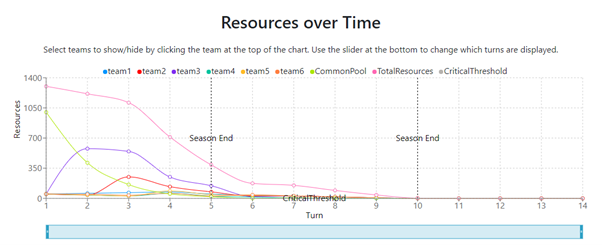
\includegraphics[scale=0.8]{12_team4_agentdesign/images/ResourcesDD.png}
\caption{Resources for Dishonest Clients Only.}
\label{fig:ResourcesDD}
\end{figure}

\subsubsection{Mixed Agents}
In an attempt to overcome the \emph{lack of variety} problem, simulations were run by instantiating two clients from each personality to promote variance. As demonstrated in Figure \ref{fig:IITOTransMA} via the “transactions” and “IITO” plots, the honest and moderate islands dominate in contributing to the community and share resources compared to the two dishonest clients “5 and 6”. Despite the clear difference in approaches from interaction plots, the game is still destined to finish early - failing to over come \emph{lack of variety}. This may be because agents are still sharing the same underlying “mindset” as they take decisions based on the same thresholds. They also are structured in the same way, so specific strategies like foraging or optional actions like proposing rules, if they are not implemented at all or just heavily relying on other clients making smart choices, will not work as well as in a more diverse environment.

\begin{figure}[H]
\centering
\begin{minipage}{.5\textwidth}
  \centering
  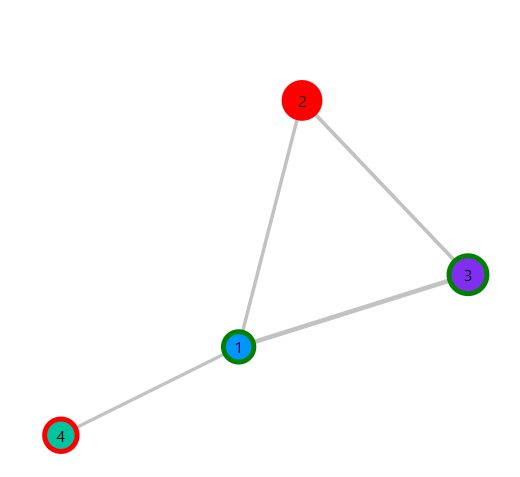
\includegraphics[width=.45\linewidth]{12_team4_agentdesign/images/IITOMA.png}
  IITO interactions
  %\captionof{IITO interactions}
\end{minipage}%
\begin{minipage}{.5\textwidth}
  \centering
  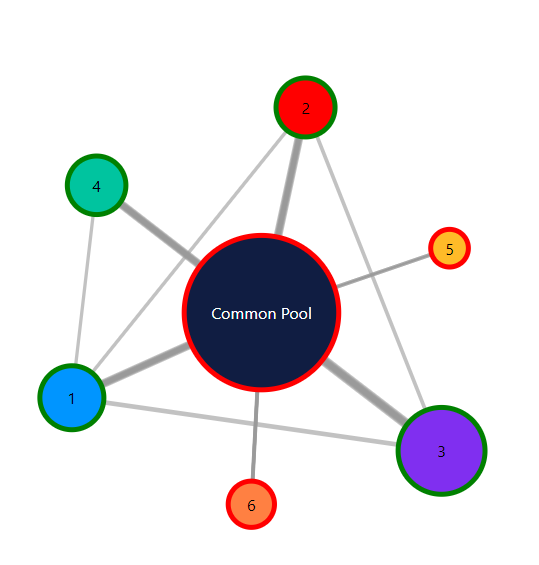
\includegraphics[width=.45\linewidth]{12_team4_agentdesign/images/TransactionsMA.png}
  Transactions
  %\captionof{Transactions}
\end{minipage}
  \label{fig:IITOTransMA}
  \caption{IITO interactions and transactions among mixed clients.}
\end{figure}


\subsection{Results Summary} \label{ResultSummary}
%Rudolfs suggestion on phrasing it as experts in the field allow all islands to thrive.%
\subsubsection{Lack of variety}
The \emph{lack of variety} problem was a reoccurring trend in all uni-agent systems. The question comes in when considering whether or not this trend was avoidable or not. Because the agents had a limited number of actions it could take, putting the same strategies up against each other resulted in a stalemate due to the lack of variance. By theory, this would be a problem regardless of what the specific implemented strategy actually contains.

This begs the question on whether an optimal strategy would even exist on a game such as this if all participating agents have the same level of complexity. A possible solution to this may include a more advanced state machine, an agent design our team has considered on the developing stages. The core concept is that an agent can implement different strategies accordingly to the current situation of the game state and its understanding of the other agents' strategies - a complex interpretation which would require ML components to process properly. As demonstrated by the mixed agent uni-agent simulations, making a state machine with our three agents would not have been enough variance to overcome this issue. This indicates that in order to overcome the \emph{lack of variety} problem, it is not enough to have flexible thresholds and parameters - the agent's design approach itself must be radically different at each state. This would require a lot of rewritten and well-partitioned code which was not sufficiently form-able in our limited time frame.

\subsubsection{Ostrom's Principles}
Evident by the behaviour of the dishonest agents, the tragedy of the commons was not overcome. To search for the cause of this, the system was compared with Ostrom’s principles.

A lot of Ostrom’s principles have already been enforced from the structure of the game in the form of the inter-island organisations:
\begin{enumerate}
    \item Clearly defined boundaries: The environment core infrastructure enforces the boundaries between agents.
    \item Congruence between rules and the local environment: IIGO sets different tax brackets per the agent status.
    \item Collective choice arrangements: Every agent can propose its own rules and vote existing rules off play.
    \item Monitoring by appointed agencies: The accountability cycle forms a monitoring system between the roles of power.
    \item Flexible scale of graduated sanctions: Sanctions are given in differing tiers accordingly to offences.
    \item Access to conflict resolution mechanisms: Not very applicable - discussion to be followed.
    \item Minimal recognition of right to self-organise: 
    \item System of systems: 
\end{enumerate}
In this client implementation, principle 3 is missing as the agents do not propose their own rules. Principle 6 is also missing, but this is less clear as to how this would be implemented. The way the game is made, there isn't a lot of room for conflicts to rise between islands, as the only interactions the agents have are in the form of gifts while the only form of opinions exist in the form of internal parameters which are not shared across agents.

This brings rise to the question as to whether Ostrom’s principles would be applicable to a non-ML based agent, and whether Ostrom’s rules require human behaviour as a prerequisite. Even if some rules were pre-made and given to the agents to propose and take down as the agents please, these rules wouldn't be an effect of the agents' organising - it would be an enforcement by us, the makers of the agents. One way to properly implement rule 3 would be to make the agent spontaneously create rules or create all possible rules based on its understanding of the situation of the game, which requres effective collection of all useful information from the game, as well as successful interpretation of the information. In addition, the agent would need to predict the how rules interact with each other, which is not trivial even for humans. Based on this, a further investigation of this could be done by measuring how much human influence can loom over the agents design, and its relevance to the applicability of Ostrom’s principles.


Evident by the behaviour of the dishonest agents, even with IIGO present it is still possible to completely drain the common pool from any resources. As examined in the evaluation of IIGO, there are areas of powers withing IIGO which are not governed by institutional design. One of those is a lack of a Zone of Dignity, or similar solution, for the decisions on how much the agents should request in allocations and how much the President can allocate. In the current implementation there are no rules stating that the agent is not permitted to request resource amounts above some threshold. Moreover, there are no "guardrails" the President has to follow when allocating these resources. Thus a greedy agent, like the one we implemented, in combination with a generous President results in disastrous situations, since the common pool stays permanently empty. There is no disaster mitigation and there is nowhere, besides presents, to reach for help in the case of a critical f Hence, a better approach to a dishonest agent in the current IIGO setting would be to keep all other agents minimally satisfied.
